\section{2017}
\subsection{Questions}




\subsubsection{1}

1. You are standing on a ferry travelling from Fukuoka to Busan when you drop a tennis ball into the sea. After the ball hits the water, it undergoes a deceleration until it reaches terminal velocity. Write a differential equation describing the acceleration of the ball under the water as a function of it's velocity at a given time $t$ and the terminal velocity of the ball under the water $v_T$. You may assume:
\begin{itemize}
    \item The ball falls vertically downwards.
    \item The trajectory of the ball is not disturbed by external factors such as waves or hungry fish.
    \item The density of the sea is constant so that the terminal velocity of the ball in the water is independent of depth.
    \item If you make any other assumptions, please state them clearly.
\end{itemize}

2. If the ball initially hits the water at a velocity of $2 v_T$, write an expression for the velocity of the ball as a function of time.




\subsubsection{2}

From your seat on the ferry you notice a student trying to do their homework on the Laplace equation, but they are stuck. Luckily you brought your table of Laplace transforms with you (page 3). Help the student by determining $f(t)$ in the following functions:

1. $\displaystyle \lap{f(t)} = \frac{10-10s}{s^2}$

2. $\displaystyle \lap{f(t)} = \frac{e^{-3s} s}{s^2+16}$




\subsubsection{3}

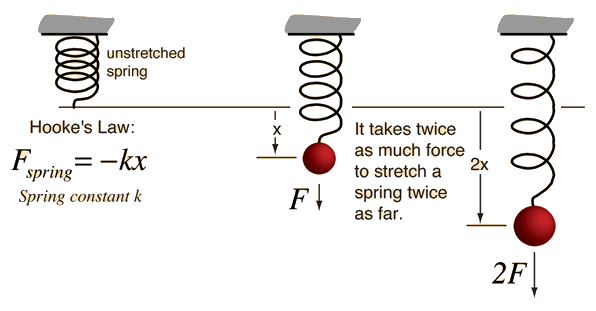
\includegraphics[width=8cm]{hooke.png}

In a play-area for children on the ferry there is a toy consisting of a mass attached to a spring hanging from the ceiling as shown in the figure above. Starting from the basic relation $F(x(t))=-kx(t)$, derive a general expression for the velocity of the mass as a function of time.




\subsubsection{4}

As you approach the port in Busan the engine of the ferry switches to reverse. During the switching, the casing of the engine vibrates with the motion described by this 2nd-order differential equation:
\begin{equation}
    3y''-4y'+y = t e^t
\end{equation}
The chief engineer wants to know the motion of the casing $y(t)$ as a function of time. Using the method of undetermined coefficients, find the general solution to this differential equation.




\newpage
\section{2016}
\subsection{Questions}
\subsubsection{1}

Solve the following ODE for $y$ given the condition $y(3)=9e^9$.

\begin{equation}
    \frac{x}{y} \frac{dy}{dx} - 1 = x^3
\end{equation}





\subsubsection{2}

The following equation is an autonamous equation:

\begin{equation}
    y'=\frac{y^2}{5}(1-\frac{y}{5})
\end{equation}
1. What key property does an autonamous equation have?


2. Determine the points of equilibrium and their stabilities.





\subsubsection{3}

Solve the following 2nd-order ODE's for $y$, and state what sort of damping they correspond to:

\begin{equation}
    y'' + 5 y' + 4y = 0 % Real
\end{equation}


\begin{equation}
    y'' + 4 y' + 4 y = 0 % Equal
\end{equation}


\begin{equation}
    y'' + 3 y' + 4 y = 0 % Complex
\end{equation}




\subsubsection{4}

Solve the following differential equation for $y$:

\begin{equation}
    3 x^2 y + 2 x y + y^3 + (x^2 + y^2) y' = 0
\end{equation}




\vspace{2cm}

\emph{Solutions can be found on the following page.}
\newpage

\subsection{Solutions}

\subsubsection{1}

$y=3xe^{x^3/3}$

\subsubsection{2}

1. $y'=f(y)$

2. $y=0$ (semi-stable), $y=5$ (stable)

\subsubsection{3}

$y(t)=C_1 e^{-t} + C_2 e^{-4t}$, Overdamped

$y(t)=C_1 e^{-2t} + C_2 t e^{-2t}$, Critically-damped

$y(t)=C_1 e^{-3t/2} Cos(\sqrt{7}t/2) + C_2 e^{-3t/2} Sin(\sqrt{7}t/2)$, Under-damped

\subsubsection{4}

$C = yx^2e^{3x} + \frac{1}{3} y^3 e^{3x}$
